	% !TEX TS-program = XeLaTeX+MakeIndex+BibTeX
% !TEX encoding = UTF-8 Unicode

\documentclass[12pt]{article}

%\usepackage[utf8]{inputenc}
\usepackage[brazilian]{babel}

\usepackage{fontspec}
\setmainfont{Linux Libertine G}
\linespread{1.05}

%%% PAGE DIMENSIONS
\usepackage{geometry} % to change the page dimensions
\geometry{a4paper} % or letterpaper (US) or a5paper or....
% \geometry{margin=2in} % for example, change the margins to 2 inches all round
% \geometry{landscape} % set up the page for landscape

\usepackage{graphicx} % support the \includegraphics command and options

% \usepackage[parfill]{parskip} % Activate to begin paragraphs with an empty line rather than an indent

%%% PACKAGES
\usepackage{amsfonts}
\usepackage{color}
%\usepackage{booktabs} % for much better looking tables
%\usepackage{array} % for better arrays (eg matrices) in maths
%\usepackage{paralist} % very flexible & customisable lists (eg. enumerate/itemize, etc.)
\usepackage{verbatim} % adds environment for commenting out blocks of text & for better verbatim
\usepackage{microtype}
\usepackage[numbers]{natbib}
%\usepackage{subfig} % make it possible to include more than one captioned figure/table in a single float
% These packages are all incorporated in the memoir class to one degree or another...

\usepackage[hidelinks]{hyperref}

% For Computer Modern:
%\def\Cpp{{C\nolinebreak[4]\hspace{-.05em}\raisebox{.4ex}{\tiny\bf ++}}}
% For Linux Libertine G
\def\Cpp{{C\nolinebreak[4]\raisebox{.20ex}{\small\bf++}}}

\newcommand{\todo}[1]{\textsf{\color{red}#1}}

%%% END Article customizations

\title{Desenvolvimento e Reutilização de Testes Automatizados em Aplicações Web}
\author{Lucas Antunes Amaral \\ \emph{Universidade Federal de Santa Maria}}
%\date{} % Activate to display a given date or no date (if empty), otherwise the current date is printed 

\begin{document}
	\maketitle
	
	\section{Identificação}
	
	\begin{description} \itemsep 0pt
		\item[Resumo:] ~\\
		A constante busca pela qualidade de uma solução em forma de software, fez com que empresas do ramo de desenvolvimento,
		aderissem e enxergassem a importância da realização de testes automatizados em seus sistemas. A partir deste cenário,
		surgiram inúmeras ferramentas e frameworks para suprir esta demanda, que se propõe  a ampliar a otimização de tempo e
		eficácia das aplicações implementadas, visando uma garantia maior na qualidade das mesmas. Contudo, é sabido que criar
		um novo teste para cada nova funcionalidade ou demanda do sistema, se torna muito custoso, sendo necessário um grande
		desprendimento de recursos humanos. Assim, este trabalho objetiva apresentar scripts de testes automatizados para
		sistemas web, que possam, de maneira mais genérica e com poucas alterações, serem reutilizados, de forma escalável,
		para novos casos de testes, que sigam o mesmo escopo.
		\item[Período de execução:] Agosto de 2015 a Dezembro de 2015
		\item[Unidades participantes:] ~\\ Curso de Ciência da Computação
		\item[Área de conhecimento:] Ciência da Computação
		\item[Linha de Pesquisa:] Linguagens de Programação, Qualidade de Software, Testes de Software
		\item[Tipo de projeto:] Trabalho de Conclusão de Curso
		\item[Participantes:] ~\\ Profª Andrea Schwertner Charão -- Orientadora \\ Lucas Antunes Amaral -- Orientando
	\end{description}
	
	\section{Introdução}
	
	Dada a atual conjectura do mercado de desenvolvimento de software, é fundamental para
	que uma aplicação se mantenha viva de forma competitiva, apresentar diferenciais ao seu público alvo. Desta
	maneira a área de qualidade de software ganha cada vez mais espaço dentro das empresas de TI e, em especial, as ferramentas e
	metodologias de teste de software ganham maior visibilidade.
	
	Os testes de software podem ocorrer em todas as etapas do desenvolvimento e de diferentes formas, contudo,
	sempre objetivam atender na totalidade os requisitos do sistema e, simultaneamente, amplificar a qualidade da solução
	codificada. São inúmeras as vantagens de se utilizar testes automatizados ao invés dos testes manuais em uma aplicação.
	Apesar de, aparentemente, ser mais prático e rápido realizar um teste manual, a cada nova alteração em um módulo do sistema,
	o teste tem que ser todo refeito e a tendência que novos erros sejam gerados até mesmo em funcionalidades já testadas é enorme,
	problema este que não ocorre quando a abordagem escolhida é a automatização dos testes.
	
	Mesmo apresentando grandes vantagens, os testes automatizados demandam um grande custo inicial em sua codificação e, com isso, aumenta o 
	envolvimento da equipe de qualidade. Pensando nesse problema, podemos buscar formas alternativas para
	que se possa usufruir de todas estas virtudes dos testes automatizados, e, ao mesmo tempo, utilizar de forma eficiente os
	recursos disponíveis em uma instituição.
	
	\section{Objetivos}
	
	\subsection{Objetivo Geral}
	
	Este trabalho tem como objetivo principal apresentar um conjunto de casos de teste e testes que possam ser reutilizados de
	forma otimizada em novas funcionalidades de uma aplicação ou em sistemas que sigam os mesmos padrões e comportamento dos
	softwares conhecidos.
	
	\subsection{Objetivos Específicos}
	\begin{itemize}
		\item Apontar diferenças de casos de testes;
		\item Gerar testes automatizados reaplicáveis em novos casos;
		\item Gerar casos de testes genéricos para um escopo definido.
	\end{itemize}
	
	\section{Justificativa}
	
	A qualidade de software  é uma das variáveis essenciais para que um projeto de software tenha sucesso.
	Sendo assim, torna-se cada vez mais necessário a inserção de testes automatizados em projetos web,
	agregando aos mesmos uma maior confiabilidade e redução nos possíveis erros que o sistema possa
	apresentar. Para que haja a possibilidade de aumentar a qualidade dos sistemas, sem que seja necessário uma maior
	demanda de recursos humanos para a área de qualidade, podemos adotar práticas de reuso de códigos de testes, visando
	maximizar a produtividade e eficiência, além de, simultaneamente, obter um produto final com uma garantia de qualidade
	superior.
	
	\section{Revisão de Literatura}

	Abaixo, serão apresentados conceitos relativos os conteúdos abordados neste trabalho, descrevendo, qualidade de software, ferramentas de teste de software, assim como o reuso de testes.
	
	\subsection{Qualidade de Software}
	
	A Qualidade de software é uma subárea oriunda da engenharia de software, que tem com foco central apresentar metodologias,
	procedimentos e métricas que garantam a qualidade no processo de desenvolvimento de um sistema. Apesar de ocorrer no processo, a Qualidade de software
	objetiva obter qualidade no produto final, e, com isso, consiga contemplar na totalidade os requisitos tratados com o cliente ao longo do processo.
    \citeauthor{de2006introduccao} \cite{de2006introduccao} afirma que a qualidade de software está diretamente relacionada a um gerenciamento
    rigoroso de requisitos, uma gerência efetiva de projetos e em um processo de desenvolvimento bem definido, gerenciado e em melhoria contínua. Afirma também,
    que atividades de verificação e uso de métricas para controle de projetos e processo também estão inseridas nesse contexto, contribuindo para tomadas de
    decisão e para antecipação de problemas.

    Mas como medir a qualidade de um sistema em questão? Para responder este questionamento, Garvin \cite{garvin1987competing} propõe o conceito que ele chama de
    oito dimensões, que seriam em ordem, qualidade do desempenho, qualidade dos recursos, confiabilidade, conformidade, durabilidade, facilidade de manutenção,
    estética e percepção. Segundo \citeauthor{garvin1987competing}, atendendo a estes oito critérios, o sistema apresentará qualidade.
    \citeauthor{pressman2011engenharia} \cite{pressman2011engenharia} complementa a definição de Garvin mesclando-a com a norma ISO 9126, e aponta os fatores
    críticos para o sucesso neste caso, como sendo: Intuição, Eficiência, Robustez e Riqueza.

	
	\subsubsection{Qualidade do processo}
	
	A qualidade de software é largamente determinada pela qualidade dos processos utilizados para o desenvolvimento. Deste modo, a melhoria 
	da qualidade de software é obtida pela melhoria da qualidade dos processos \cite{koscianski2007qualidade}. 
	
	\subsubsection{Qualidade do produto}

	Existe uma relação direta entre qualidade de produto e qualidade do processo, pois, para obtenção da qualidade do produto final,
	faz-se necessário adquirir primeiramente qualidade nos processos que compõem o desenvolvimento do mesmo.
	Avaliar a qualidade de um produto de software é verificar, através de técnicas e atividades operacionais o quanto os requisitos são atendidos. Tais requisitos,
	de uma maneira geral são a expressão das necessidades, explicitados em termos quantitativos ou qualitativos, e têm por objetivo definir as características de
	um software, a fim de permitir o exame de seu atendimento \cite{koscianski2007qualidade}.
	
	\subsubsection{Testes de Software}

	É a atividade responsável por apresentar os erros existentes em um determinado programa, por isso, pode ser vista como uma atividade destrutível, pois visa expor os defeitos para depois corrigir os mesmos, e, de preferência, em um estágio inicial. Quanto mais tarde um defeito for identificado mais caro fica para corrigi-lo e mais, os custos de descobrir e corrigir o defeito no software aumentam exponencialmente na proporção em que o trabalho evolui através das fases do projeto de desenvolvimento \cite{boehm1976quantitative}. O teste possibilita também, validar se os requisitos inicias do sistema, alinhados pelos \emph{stakeholders}, estão contemplados em sua plenitude.

	Apesar de não ser possível, através de testes, provar que um programa está correto, os testes, se conduzidos sistemática e criteriosamente, contribuem para aumentar a confiança de que o software desempenha as funções especificadas e evidenciar algumas características mínimas do ponto de vista da qualidade do produto \cite{maldonado2004introduccao}. Sendo assim, se faz essencial o mapeamento de um processo de testes para que se possa criar garantias e métricas que reduzam os erros, maximizando a qualidade, \citeauthor{crespo2004metodologia} \cite{crespo2004metodologia} descreve o processo de teste, como sendo a composição de quatro macro etapas: Planejamento, projeto, execução e acompanhamento dos testes de unidade.

	\subsubsection{Estratégias de Testes}
	A Estratégia de testes se caracteriza pela definição da abordagem geral a ser aplicada nos testes, descrevendo como o software será testado, identificando os níveis de testes que serão aplicados, os métodos, técnicas e ferramentas a serem utilizada \cite{rios2006teste}. Existem muitas estratégias mas podemos destacar entre elas: Teste de unidade, integração, sistema, aceitação e regressão, funcional e carga. Se pode também, mesclar mais de uma estratégia com o intuito de reduzir os possíveis defeitos que o sistema venha a ter.	

	\subsection{Ferramentas para teste de software}
	Existem muitas ferramentas desenvolvidas para realização de testes de software web, neste trabalho serão descritas duas(2) dentre elas, que serão as ferramentas utilizadas no desenvolvimento dos testes estudados.

	\subsubsection{Cucumber}
	Cucumber é um ferramenta de desenvolvimento de testes, voltado para sistemas web, que adota uma linguagem de alto nível bem próxima à uma linguagem natural e tem suas origens fixadas sobre a metodologia BDD (Behavior Driven Development). Cucumber é escrita em linguagem Ruby, mas pode ser utilizada para executar especificações de aplicações escritas em qualquer linguagem \cite{nunescucumber}. 

	A escolha dessa ferramenta, baseou-se na fácil transcrição dos requisitos do sistema para a linguagem em questão, tornando possível conferir se os requisitos estão contemplados pelas funções e métodos descritos no sistema \emph{web}. \citeauthor{lopescucumbervalor}\cite{lopescucumbervalor} compara Cucumber com o \emph{software} Capybara e afirma que o primeiro apresentar um código mais legível e amigável. Uma observação é que o código com Capybara faz referência para vários detalhes de implementação, enquanto o código do Cucumber reserva isso apenas para os \emph{Steps} e não para o arquivo de feature \cite{lopescucumbervalor}. 

	A ferramenta funciona basicamente através da leitura de arquivos com a extensão feature, os quais descrevem em linguagem natural uma funcionalidade e casos de teste, conhecidos como cenários.     
	Como os testes estão escritos em uma linguagem natural, e não de programação, Cucumber precisa pesquisar pelo código associado aos passos que formam o cenário em arquivos auxiliares \cite{scmitzcucumberreview}. Cucumber executa seus arquivos \emph{.feature}, e esses arquivos contêm especificações executáveis escritos em uma linguagem chamada Gherkin \cite{cucumberwiki}, que, possui um layout bem definido. Inicia pela descrição de uma funcionalidade, que por sua vez possui cenários, onde, um cenário é descrito da seguinte forma: \emph{Dado} alguma condição \emph{Quando} outra condição \emph{E} terceira condição \emph{Então} faça algo, conforme ilustra a figura \ref{fig:codigo_cucumber}.

	\begin{figure}[!htb]
		\centering
		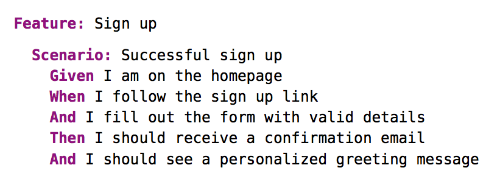
\includegraphics[width=0.8\textwidth]{codigo_cucumber}
		\caption{Um exemplo de código cucumber.}
		\label{fig:codigo_cucumber}
	\end{figure}

	\subsubsection{Selenium HQ}
	É um framework open source, utilizado para automatização de testes funcionais em aplicações web \cite{chiavegatto1desenvolvimento}. Segundo \citeauthor{pereiraestudoselenium} \cite{pereiraestudoselenium}, se trata
	de uma ferramenta de fácil uso e eficiente para desenvolver casos de teste, permitindo os testes de aceitação ou funcional, regressão e de desempenho.
	Selenium trabalha como um plugin do navegador Firefox, o mesmo traz muita praticidade pois permite que se possa capturar cliques e valores digitados transformando-os em um caso de teste. Ele é composto por
	quatro ferramentas: Selenium IDE, Selenium Grid, Selenium RC e Selenium WebDrive.

	A  utilização  de  comandos  no  Selenium  consiste  em  digitar  o  comando  seguido  de  dois parâmetros  tal  como  por  exemplo \emph{verifyText //div//a[2] Login}. Dependendo  do  comando,  os parâmetros
	poderão ser opcionais, aliás, alguns comandos não necessitam de parâmetros para serem executados \cite{sixpenceautomatizaccao}.

	Selenium foi escolhida como umas das ferramentas no desenvolvimento deste projeto pelo fato de ser um \emph{framework open source} que possui um vasto leque de ferramentas para testes de sistemas web. Outro fator
	importante para sua escolha, é a possibilidade de interação do Selenium HQ com o Cucumber. Ela  se  destaca  entre  as demais ferramentas  gratuitas pelo fato de ser a mais completa, permitindo integração com
	várias linguagens,  outros \emph{frameworks}, além de suportar inúmeros navegadores e sistemas operacionais \cite{pereiraestudoselenium}.

	\subsection{Reuso de testes}

	Visando melhor aproveitar os recursos existentes em uma instituição e ainda assim apresentar garantias na qualidade do produto/serviço entregues aos clientes, desenvolvedores do mundo todo, começaram a apresentar
	teses e modelos que buscam criar testes genéricos e padronizados. Um padrão é um pedaço de informação instrutiva e nomeada, que captura a estrutura essencial
	e \emph{“insights”} de uma família bem sucedida de soluções aprovadas para um determinado problema, o qual surge em um determinado contexto \cite{cagnin2004reuso}.

	\citeauthor{guizzardi2000desenvolvimento} diz que por razões histórias a área de desenvolvimento de software não atingiu a maturidade que outras áreas da engenharia atingiram, complementa afirmando,
	que apesar disso, é inegável que algum avanço tenha sido alcançado, pois a forma de realização dessa atividade evoluiu de uma atividade realizada de forma quase artesanal, para um processo de
	desenvolvimento bem estruturado e que, nos melhores casos, contempla inclusive atividades de gerência e avaliação da qualidade \cite{guizzardi2000desenvolvimento}.
	Com isso, a reutilização dos testes já codificados, se mostra uma importante prática no desenvolvimento e que ainda apresenta muitas incógnitas e possibilidades para as equipes de TI,
	principalmente na geração de casos de testes que possam ser reutilizados em situações que apresentem um padrão parecido com os casos já conhecidos.

	\section{Metodologia}

	O projeto em questão, se trata de um trabalho exploratório, onde o mesmo será dividido em três(3) grandes fases, que seriam:

	\subsection{Planejamento dos testes necessários}
	Fase na qual serão elencados potenciais classes que necessitam de maiores cuidados nos sistemas escolhidos, será também, o momento onde ocorrerá o mapeamento dos casos de testes necessários que deverão ser
	desenvolvidos nas fases seguintes deste projeto.

	\subsection{Programação dos testes automatizados}
	Momento no qual serão escritos os códigos dos testes planejados na primeira fase do projeto, utilizando Selenium HQ e Cucumber como ferramentas para codificação dos mesmos.

    \subsection{Análise e geração de casos de teste reutilizáveis}
    Última etapa do projeto, responsável pela geração de \emph{scripts} que contenham testes que possam ser reaproveitados em novas situações e funcionalidades para aplicações web que sigam o mesmo perfil das
    aplicações para os quais os mesmos foram criados.

	\section{Plano de Atividades e Cronograma}

	O cronograma de atividades será composto de 5 etapas, são elas:
	
	\begin{enumerate}
		\item \label{activity:configuracao} \textbf{Configuração e estudo sobre \emph{Selenium HQ} e \emph{Cucumber}:}
		Nesta etapa, ocorrerá os devidos estudos sobre as ferramentas escolhidas para
		desenvolvimento deste trabalho, assim como a instalação das mesmas.
		\item \label{activity:desenvolvimento_1} \textbf{Desenvolvimento de testes 1º software:}
		Trata-se de elencar alguns testes necessários no primeiro software selecionado para o desenvolvimento,
		e após, codificá-los.
		\item \label{activity:desenvolvimento_2} \textbf{Desenvolvimento de testes 2º software:}
		Desenvolvimento de testes para o segundo software web deste projeto.
		\item \label{activity:analise} \textbf{Análise das similaridades dos testes desenvolvidos:}
		Análise das diferenças e igualdades dos testes desenvolvidos sobre os dois sistemas web selecionados,
		elencando um padrão que possa ser reutilizado.
		\item \label{activity:final} \textbf{Confecção de rotinas e testes genéricos para aplicações web:}
		Codificação de testes padronizados, que possam ser utilizados em grande parte e com poucas alterações,
		em outros projetos que sigam o mesmo padrão que os estudados neste trabalho.
	\end{enumerate}

	\begin{table}[ht]
		\centering
		\begin{tabular}{c|ccccc}
			Etapa & Agosto & Setembro & Outubro & Novembro & Dezembro \\ \hline
			\ref{activity:configuracao} & \checkmark & \checkmark & & & \\
			\ref{activity:desenvolvimento_1} & & \checkmark & \checkmark & & \\
			\ref{activity:desenvolvimento_2} & & \checkmark & \checkmark & & \\
			\ref{activity:analise} & & & \checkmark & \checkmark & \\
			\ref{activity:final} & & & & &\checkmark \\
		\end{tabular}
		\caption{Cronograma de Atividades}
	\end{table}
	
	\section{Recursos}
	
	Como recursos físicos, serão utilizados neste trabalho, apenas o computador pessoal do pesquisador juntamente
	com ferramentas open source para teste de software web, que serão instaladas no mesmo.
	
	\section{Resultados Esperados}
	
	Ao término deste projeto, espera-se obter como resultado um conjunto de testes e casos de testes genéricos,
	que possam ser aplicados em um software web que possua características similares aos softwares utilizados
	nesta pesquisa.
	
	\bibliographystyle{abbrvnat}
	\bibliography{../referências}
	
\end{document}